\documentclass[a4paper,11pt]{ltjsarticle}

\usepackage[top=24mm,bottom=25mm,left=24mm,right=24mm]{geometry}
\usepackage[haranoaji,nfssonly]{luatexja-preset}
\usepackage{amsmath,amssymb,bm}
\usepackage{booktabs}
\usepackage{array}
\usepackage{graphicx}
\usepackage{float}
\usepackage{tikz}
\usetikzlibrary{arrows.meta,positioning,shapes.geometric}
\usepackage{enumitem}
\usepackage{xcolor}
\usepackage{hyperref}
\usepackage{xurl}
\usepackage{xspace}

\hypersetup{
  colorlinks=true,
  linkcolor=blue!45!black,
  citecolor=blue!45!black,
  urlcolor=blue!55!black,
  pdftitle={MassivelyによるBoltzmann Particle HydrodynamicsのポータブルGPU実装},
  pdfauthor={Akira Hayakawa}
}
\graphicspath{{../workspace/plot/}}
\setlength{\emergencystretch}{3em}
\setlist{nosep}

\newcommand{\bphgpu}{\texttt{bph-gpu}\xspace}
\newcommand{\massively}{\texttt{massively}\xspace}
\newcommand{\cubecl}{CubeCL\xspace}
\newcommand{\vect}[1]{\bm{#1}}
\newcolumntype{L}[1]{>{\raggedright\arraybackslash}p{#1}}

\title{Massivelyによる\\
Boltzmann Particle HydrodynamicsのポータブルGPU実装}
\author{Akira Hayakawa}
\date{2026年7月18日}

\begin{document}
\maketitle

\begin{abstract}
粒子法は、数値流体力学に対して相補的な計算手段を提供する。Smoothed
Particle Hydrodynamics（SPH）は、近傍の物質粒子間のカーネル重み付き相互作用に
よって連続体方程式を離散化する。一方、Boltzmann Particle
Hydrodynamics（BPH）は、速度分布をMonte Carlo粒子で表現し、自由飛行と直交格子
セル内の確率的緩和を交互に行う。BPHは高Mach数流れや真空を扱う上で魅力的で
あるが、標本ゆらぎを抑えるには多数の粒子が必要であり、高いメモリスループット
が要求される。本論文では、\massively v0.80と \cubecl カーネル言語に基づく
Rust製のポータブルGPU実装 \bphgpu を示す。中心的な実装課題は、緩和がセル局所
である一方、セル粒子数が不均一で自由飛行ごとに変化し、更新後の状態は粒子単位
で対応を保って書き戻す必要があることである。この不整合をsort-by-key、
reduce-by-key、scatter、gather、masked transform、stream compactionの合成に
よって解決する。これらの操作は、セルごとの逐次ループや競合するatomic加算を
使わず、セル局所緩和を規則的な粒子配列とセル配列上の処理へ変換する。緩和更新を
導出し、GPU実装に必要な順序・データ配置の不変条件を示すとともに、再実装可能な
粒度で並列プリミティブ列を記述する。演算子テストとSod衝撃波管計算を簡潔な実装
実証として示す。本論文の焦点はGPUへの写像であり、BPHの新たな物理検証や特定
deviceに対するbenchmark上の主張ではない。
\end{abstract}

\begin{center}
\small
\textbf{キーワード：} Boltzmann Particle Hydrodynamics、Smoothed Particle
Hydrodynamics、GPU、Rust、並列プリミティブ、Monte Carlo粒子法
\end{center}

\section{序論}

粒子法は数値流体力学において長い歴史を持つ。SPHは天体物理学的な気体力学を
対象として、LucyとGingold--Monaghanにより独立に導入された
\cite{lucy1977,gingold1977}。SPHは移動する物質粒子によって連続体を表現し、場と
その勾配を、近傍粒子上のコンパクト台カーネル和で近似する。このLagrange的かつ
mesh-freeな記述は、大変形、移動界面、自由表面に対して特に有効である
\cite{monaghan1992}。

これと相補的な発展は気体分子運動論から始まる。Direct Simulation Monte
Carlo（DSMC）は、分子速度分布をsimulation粒子で表現し、決定論的な移動と確率的
衝突を分離する \cite{bird1994}。Isaka、Matsuda、Boffinはこの考えをMolecular
Hydrodynamics（MH）として連続体気体流れへ適用し、内部自由度、衝撃波、真空、
高Mach数状態を扱った \cite{isaka2006}。その後Murataらは、この連続体粒子scheme
の安定性と時間刻み依存性を解析した \cite{murata2008}。日本流体力学会年会講演論文
集に発表された後続研究ではBPHという名称が用いられ、可変粒子数および可変重みが
検討された \cite{isaka2010}。本論文で扱うBPHは同じstream--relax構造に従うが、
明示的な分子衝突を、Boltzmann方程式のBGK近似に基づくセル局所緩和に置き換える
\cite{bgk}。

したがってSPHとBPHはいずれもLagrange的粒子法として関連するが、同じ離散化では
ない。SPH粒子は連続体方程式に対する移動求積点として働き、平滑化カーネルを介して
相互作用する。BPH粒子は位相空間分布を標本化し、固定セルが緩和を局所化する。
密度、bulk速度、圧力は粒子集団のmomentとして復元される。自由飛行では、1回の
更新でBPH粒子が複数セルを横断できる。このため通常の陽解法格子におけるCFL限界を
超えても安定な計算が可能である。ただし、大きな時間刻みは分離誤差と数値粘性を
通じて精度を低下させる \cite{isaka2006,murata2008}。

粒子表現では、密度が非負の粒子数から、熱エネルギーが非負の運動エネルギーと
内部エネルギーから得られるため、極端な状態を扱いやすい。主な代償はMonte Carlo
noiseである。$N_g$個の粒子を含むセルでは、通常の標本誤差は
$O(N_g^{-1/2})$で減少する。誤差を10分の1にするには約100倍の標本が必要となる。
したがって、メモリ容量とスループットが中心的な課題になる。

関連する粒子法のGPU研究から、有用な計算patternが得られている。GPU高速化SPHは
空間セル、粒子の並べ替え、近傍処理、device上の時間積分を用いて数百万粒子を扱う
\cite{crespo2011}。全処理をdevice上で行うDSMC実装も、粒子移動、セル番号計算、
衝突、標本化を並列化する \cite{su2012}。BPHにも同様にdata parallelismを利用する
余地があるが、そのセル緩和に必要なのは、SPHのカーネル力評価やDSMCの粒子対衝突
選択ではなく、segmentごとの集約と再配布である。

本研究では、\massively v0.80と \cubecl を基盤としてRustで \bphgpu を開発する
\cite{massively,cubecl}。主題は、BPHをGPU上で実行するために必要なアルゴリズム
上の写像である。本論文の貢献は3点である。第1に、等質量と完全緩和という仮定を
含め、並列実装が保存すべき数学的更新を明示する。第2に、time stepごとに変わる
セル所属、著しく不均一なセル粒子数、粒子データとセルデータの変換、空セル、全粒子
場へ同じ並べ替えを適用する必要性、というGPU固有の課題を整理する。第3に、
\massively の公開並列プリミティブを使い、各課題をdevice上の配列操作のポータブル
な合成として表現する方法を示す。衝撃波管は、合成した実装が意図したBPH cycleを
実行することの実証としてのみ用い、包括的な物理検証とは位置付けない。

\section{理論的背景}

\subsection{BGK方程式と演算子分割}

$\vect{x}$を位置、$\vect{c}$を分子速度、$\vect{F}$を外力加速度、$n$を数密度、
$f$を規格化された速度分布とする。BGK方程式は
\begin{equation}
 \frac{\partial(nf)}{\partial t}
 + \vect{c}\cdot\nabla_{\vect{x}}(nf)
 + \vect{F}\cdot\nabla_{\vect{c}}(nf)
 = n\frac{f^{\mathrm{eq}}-f}{\tau},
 \label{eq:bgk}
\end{equation}
である。ここで$\tau$は緩和時間である \cite{bgk}。BPHで用いる平衡分布の代替
$f^{\mathrm{eq}}$はMaxwell分布である必要はない。速度空間で等方的であり、質量、
運動量、全エネルギーのmoment
\begin{equation}
 \int nf\,Q(\vect{c})\,d\vect{c}
 =\int nf^{\mathrm{eq}}\,Q(\vect{c})\,d\vect{c},
 \quad
 Q\in\left\{m,m\vect{c},\tfrac12m|\vect{c}|^2+e\right\}.
 \label{eq:moments}
\end{equation}
を保存すれば十分である。本論文で調べる実装は、この平衡分布代替の角度成分に
球殻分布を用いる。

式~\eqref{eq:bgk}を輸送と衝突に分割する。概念的には、1 time stepは
\begin{equation}
 \text{streaming: }(\vect{x},\vect{c})\longrightarrow
 (\vect{x}^{*},\vect{c}^{*}),
 \qquad
 \text{relaxation: }f^{*}\longrightarrow f^{n+1}.
\end{equation}
となる。数値解法では図~\ref{fig:loop}に示す順序、すなわちセル番号計算、粒子の
並べ替え、緩和、streaming、境界条件の適用を反復する。ある反復で得られた位置を
次の反復の緩和が用いるため、この順序とmove--then--relaxという記述との差は時間
labelだけである。外力がない場合、1次精度のstreaming更新は
\begin{equation}
 \vect{x}^{n+1}=\vect{x}^{n}+\vect{c}^{n+1}\Delta t.
 \label{eq:stream}
\end{equation}
である。第4節の数値実証では外力を用いない。

\begin{figure}[H]
 \centering
 \begin{tikzpicture}[
   node distance=7mm,
   box/.style={draw,rounded corners,minimum width=46mm,minimum height=8mm,
               align=center,fill=blue!5},
   arr/.style={-{Latex[length=2.2mm]},thick}
 ]
  \node[box] (index) {セル番号を計算\\粒子ごとのtransform};
  \node[box,below=of index] (sort) {セルkeyと粒子状態を同時にsort};
  \node[box,below=of sort] (relax) {セルreductionとgather\\BPH緩和};
  \node[box,below=of relax] (move) {自由飛行（RK1）};
  \node[box,below=of move] (bound) {反射・周期・流出境界};
  \draw[arr] (index) -- (sort);
  \draw[arr] (sort) -- (relax);
  \draw[arr] (relax) -- (move);
  \draw[arr] (move) -- (bound);
  \draw[arr] (bound.east) -- ++(13mm,0) |- (index.east);
 \end{tikzpicture}
 \caption{BPHの1 time step。GPU実装では、loop全体を通じて粒子状態をdevice上に
 保持する。}
 \label{fig:loop}
\end{figure}

\subsection{粒子状態、比熱比、および前提条件}

粒子$i$は、位置$\vect{x}_i$、速度$\vect{c}_i=(u_i,v_i,w_i)$、質量$m_i$、
内部エネルギー$e_i$、セル番号$g(i)$を持つ。3つの並進自由度に加えて、粒子は
$s\geq0$個の内部自由度を持つ。対応する比熱比は
\begin{equation}
 \gamma=1+\frac{2}{3+s}=\frac{s+5}{s+3}.
 \label{eq:gamma}
\end{equation}
である。したがって$s=0$では$\gamma=5/3$、$s=2$では$\gamma=7/5$となる。

ここで扱う定式化では、1つの緩和に参加する粒子の質量と$s$が等しいと仮定する。
粒子質量が異なる場合、式~\eqref{eq:center}の算術平均を質量重み付き平均に置き換える
必要がある。したがって、以下の保存則の導出と数値実証では$m_i=m$と仮定する。

\subsection{単一セル内の緩和}

$I_g$をセル$g$に属する粒子の集合、$N_g=|I_g|$とする。$N_g<2$のセルでは衝突を
model化できないため、状態を変更しない。$N_g\geq2$の場合、平均速度と熱速度を
\begin{equation}
 \vect{U}_g=\frac{1}{N_g}\sum_{i\in I_g}\vect{c}_i,
 \qquad
 \vect{q}_i=\vect{c}_i-\vect{U}_g.
 \label{eq:center}
\end{equation}
と定義する。重心系で再配分されるエネルギーは
\begin{equation}
 E_g=\sum_{i\in I_g}
 \left(\frac12m|\vect{q}_i|^2+e_i\right).
 \label{eq:cellenergy}
\end{equation}
である。エネルギー等分配則により、緩和後の並進運動エネルギーと内部エネルギーを
$3:s$の比で
\begin{equation}
 K_g^{\star}=\frac{3}{3+s}E_g,
 \qquad
 E_{\mathrm{int},g}^{\star}=\frac{s}{3+s}E_g.
 \label{eq:partition}
\end{equation}

に配分する。各粒子について、2つの独立な一様乱数
$r_{1i},r_{2i}\in[0,1)$から
\begin{align}
 \mu_i &= 1-2r_{1i}, & \theta_i&=2\pi r_{2i},\\
 \vect{d}_i &=
 \left(\sqrt{1-\mu_i^2}\sin\theta_i,
       \sqrt{1-\mu_i^2}\cos\theta_i,\mu_i\right).
 \label{eq:shell}
\end{align}
を生成する。$|\vect{d}_i|=1$であるため、これらのvectorは単位球面上に一様分布
する。有限標本のvector和は厳密には0にならないので、セルごとに
\begin{equation}
 \widehat{\vect{d}}_i=\vect{d}_i-
 \frac{1}{N_g}\sum_{j\in I_g}\vect{d}_j,
 \qquad
 K_g^{\mathrm{raw}}=\sum_{i\in I_g}\frac12m
 |\widehat{\vect{d}}_i|^2.
 \label{eq:balance}
\end{equation}
としてbalanceを取る。速度scaleを
\begin{equation}
 a_g=\sqrt{\frac{K_g^{\star}}{K_g^{\mathrm{raw}}}},
 \label{eq:scale}
\end{equation}
とすると、緩和後の状態は
\begin{equation}
 \vect{c}'_i=\vect{U}_g+a_g\widehat{\vect{d}}_i,
 \qquad
 e'_i=\frac{E_{\mathrm{int},g}^{\star}}{N_g}.
 \label{eq:update}
\end{equation}
となる。式~\eqref{eq:scale}による再scaleには$K_g^{\mathrm{raw}}>0$が必要である。
連続分布から独立に方向を標本化する場合、$N_g\geq2$でこの退化事象が起こる確率は
0であるが、有限の乱数生成器では表現され得る。実装は除算をguardしてscaleを0に
する。この例外でも保存を要求する再実装では、方向を再標本化するか、和が0となる
決定論的な球殻方向をfallbackとして与える必要がある。

\subsection{保存則と数値的性質}

式~\eqref{eq:balance}より$\sum_i\widehat{\vect{d}}_i=\vect{0}$である。したがって
\begin{equation}
 \sum_{i\in I_g}m\vect{c}'_i=mN_g\vect{U}_g
 =\sum_{i\in I_g}m\vect{c}_i.
\end{equation}
となり、セルの運動量が保存される。交差項も消えるため、
\begin{align}
 \sum_{i\in I_g}\left(\frac12m|\vect{c}'_i|^2+e'_i\right)
 &=\frac12mN_g|\vect{U}_g|^2+K_g^{\star}
   +E_{\mathrm{int},g}^{\star}\\
 &=\frac12mN_g|\vect{U}_g|^2+E_g.
\end{align}
となる。よって$K_g^{\mathrm{raw}}>0$かつ厳密演算では全エネルギーも保存される。
セル緩和は粒子を生成も除去もしないため、質量保存は自明である。ただし、流出境界
では計算領域内の質量が減少し得る。

BGK衝突項をforward Euler離散化すると、緩和確率$P=\Delta t/\tau$を導入できる。
粘性流では、この確率で緩和を標本化することにより有限の平均自由行程を表現できる。
一方、$P=1$とすると、現在の \bphgpu コードが実装する完全緩和Euler modelになる。
有限$P$のNavier--Stokes粘性modelはまだ実装していない。

BPHがCFL条件に制限されないという性質は、粒子がセル境界を横断できることに由来
する。これは、任意の時間刻みで高精度であることを意味しない。$\Delta t$を増やすと
分離誤差と数値粘性が増え、境界処理では長い自由飛行中のすべての横断を整合的に
扱う必要がある。

\section{MassivelyによるGPUへの写像}

\subsection{セル緩和をGPU化する際の課題}

自由飛行は粒子局所処理であるが、緩和は純粋な粒子局所kernelでも固定幅のセル
stencilでもない。各粒子は最初に現在の所属セルを求める必要がある。1セルの粒子数
は0から全粒子の大きな割合まで変化し得る上、その分布はtime stepごとに変わる。
したがって、各セルに1 threadまたは固定workgroupを割り当てると、負荷不均衡と
必要local memory量が事前に分からないという問題が生じる。一方、各粒子に1 thread
を割り当てるだけでは、多対一の集約を行わない限り、セル和、平均、エネルギーscale
を得られない。

このため実装は、2つのindex空間を交互に扱う必要がある。長さ$N$の粒子空間は、
streaming、乱数標本化、最終状態更新に適する。長さ$K$のセル空間は、粒子数、速度
和、エネルギー、緩和scaleを保持する。実用的なGPUアルゴリズムでは、粒子値をセル
へ集約し、空セルを表現し、セル値を粒子へ再配布すると同時に、structure-of-arrays
の全列で粒子の対応を維持しなければならない。表~\ref{tab:challenges}に、
\massively v0.80によるこれらの変換をまとめる。

\begin{table}[H]
 \centering
 \small
 \caption{BPHのGPU化における課題と\massively v0.80による実現。}
 \label{tab:challenges}
 \begin{tabular}{@{}L{42mm}L{46mm}L{48mm}@{}}
  \toprule
  BPHの要件 & GPU上の課題 & Massivelyによる合成 \\
  \midrule
  現在のセル群を形成 & streaming後に所属が変化 &
  1つの共有置換による\texttt{sort\_by\_key} \\
  セルmomentを計算 & 不均一な多対一集約 &
  同一key連続区間上の\texttt{reduce\_by\_key} \\
  空セルを含める & reductionは非空keyだけを出力 &
  0初期化セル配列と\texttt{scatter} \\
  セル値を粒子へ適用 & 結果がセルindex空間に存在 &
  keyによる\texttt{gather}または等価な遅延index read \\
  衝突可能セルだけ更新 & 粒子数2未満のセルは不変 &
  masked \texttt{transform}または\texttt{gather\_where} \\
  流出粒子を除去 & 粒子数が動的に変化 &
  境界述語による\texttt{remove\_where} \\
  \bottomrule
 \end{tabular}
\end{table}

\subsection{実行modelとデータ配置}

\bphgpu は、\massively v0.80並列アルゴリズムライブラリと \cubecl カーネル言語を
用いてBPHをRustで実装する \cite{massively,cubecl}。時間積分loopの全体を通じて、
粒子データをdevice memoryに保持する。runtime抽象化により、同じアルゴリズムを
WGPU、CUDA、HIPへloweringできる。本論文の数値結果にはWGPUを用い、backend間の
等価性と性能の測定は今後の課題とする。

粒子状態$x,y,z,u,v,w,e$は、それぞれ独立した連続配列に格納する。これは
structure-of-arrays（SoA）配置である。粒子を並べ替えるすべての処理では、1つの
index置換を計算し、質量が大域定数でない場合は質量も含め、すべての状態列に同じ
置換を適用する。これにより各物理量の列は連続のままとなり、粒子ごとのcoalesced
accessが可能になる。粒子配列とセルkey配列は、常に同じ長さと粒子順序を持たなけれ
ばならない。

セル配列は空セルのentryも含め、常に長さ$K$とする。reduce-by-keyは非空セルに
対する結果だけを出力するため、このcompactな出力をセル番号に従って、0初期化した
dense配列へscatterする。次にgatherによって、各セルの値を所属粒子へ配布する。
このreduction--scatter--gather cycleが、セル局所物理量と粒子levelの並列処理を
結び付ける。

\subsection{セルkeyと順序の不変条件}

粒子数を$N$、直交格子のセル数を$K=n_xn_yn_z$とする。セル幅を$h_\alpha$、
計算領域の下端座標を$x_{\alpha,\min}$とすると、領域内部の粒子に対するセル番号は
\begin{align}
 j_{\alpha i}&=\left\lfloor
 \frac{x_{\alpha i}-x_{\alpha,\min}}{h_\alpha}\right\rfloor,
 & 0\leq j_{\alpha i}<n_\alpha,\\
 g_i&=j_{xi}+n_x\left(j_{yi}+n_yj_{zi}\right),
 &0\leq g_i<K.
 \label{eq:cellkey}
\end{align}
となる。式~\eqref{eq:cellkey}を次に評価する前に、周期境界または反射境界を越えた
座標を領域内へ戻し、流出粒子を除去しなければならない。前回の自由飛行stepで得た
keyを再利用してはならない。

key--state対を$g_i$の昇順にsortし、得られた置換をすべての粒子場へ適用する。同じ
key間のstable性は物理的要件ではない。必要な不変条件は、同一keyが連続区間を形成
し、すべての場が粒子との対応を維持することである。空間sortはGPU上のSPHおよび
DSMC実装でも標準的な構成要素である \cite{crespo2011,su2012}。

\subsection{Massivelyプリミティブの合成}

表~\ref{tab:challenges}の名称は、\massively v0.80が公開するアルゴリズムinterface、
すなわち\texttt{sort\_by\_key}、\texttt{reduce\_by\_key}、
\texttt{scatter}、\texttt{gather}、\texttt{lower\_bound}、
\texttt{upper\_bound}、masked transformに対応する。重要なのはこれらの合成であり、
ライブラリ固有のiterator型や整数変換型ではない。同じ意味の操作を提供する別のGPU
frameworkでも、同じ分解を再現できる。

順序を明示する1つの方法は、対$(g_i,i)$を第1成分でsortすることである。得られた
置換を$p$とすると、$g_{p_0}\leq g_{p_1}\leq\cdots\leq g_{p_{N-1}}$となり、すべて
の粒子場を$p$の順序でgatherする。すべての状態場へ厳密に同じ置換を適用するなら、
key--state recordを直接sortしても等価である。順序は各time stepに1回だけ計算し、
全場で共有すべきである。

中心となる再利用可能な処理はdense cell reductionである。sort済みkey
$\vect{g}$と粒子値$\vect{a}$を与えると、reduce-by-keyはまず、非空セルの一意な
key $\vect{\kappa}$とcompactな和$\vect{s}$を返す。これらを0初期化したセル配列へ
scatterすると、
\begin{equation}
 (\vect{\kappa},\vect{s})=\operatorname{reduce\_by\_key}
 (\vect{g},\vect{a}),\qquad
 \vect{A}=\vect{0}_K,\qquad
 A_{\kappa_j}\leftarrow s_j.
 \label{eq:densereduce}
\end{equation}
となる。この構成は、競合する粒子--セル間atomic加算を使わずに、空セルを明示的に
表現する。セル$g$の粒子数は、sort済みkey配列における$g$のupper boundとlower
boundの差である。これと等価に、全要素が1の粒子配列へ
式~\eqref{eq:densereduce}を適用しても求められる。

任意のdenseセル場$A_g$に対し、粒子keyによる置換から粒子場$a_i=A_{g_i}$を構成
する。GPU実装では、このindex readを消費側kernelへ融合しても、gather後の粒子
配列を実体化してもよい。両者の数学的意味は同じである。SoA場の対応を維持する
限り、$(u,v,w)$のようなvector量は成分ごとに処理してもtupleとして処理してもよい。
$N_g\geq2$というmaskで緩和対象粒子を選び、それより小さいセルの粒子は以前の状態
を保持する。

\subsection{並列緩和}

以下の手順により、完全緩和BPHの衝突stepを再実装できる。ここで
\textsc{DenseReduce}は式~\eqref{eq:densereduce}、
\textsc{Gather}$(A,\vect{g})_i=A_{g_i}$を表し、すべての粒子mapは並列である。
\begin{enumerate}[label=\arabic*.]
 \item $N_g$と$\vect{S}_g=\textsc{DenseReduce}(\vect{g},\vect{c})_g$を計算し、
       非空セルについて$\vect{U}_g=\vect{S}_g/N_g$を求める。
 \item $\vect{U}_{g_i}$をgatherして緩和の最後まで保存し、各速度を中心化する：
       $\vect{q}_i=\vect{c}_i-\vect{U}_{g_i}$。
 \item 次を計算する：
       $E_g=\textsc{DenseReduce}\bigl(\vect{g},
       \tfrac12m|\vect{q}|^2+e\bigr)_g$.
 \item 2つの独立な一様乱数粒子配列を生成し、式~\eqref{eq:shell}でtransformして
       $\vect{d}_i$を得る。
 \item 次を計算する：
       $\overline{\vect{d}}_g=
       \textsc{DenseReduce}(\vect{g},\vect{d})_g/N_g$。さらに
       $\widehat{\vect{d}}_i=\vect{d}_i-
       \overline{\vect{d}}_{g_i}$。期待値としての等方性だけでなく、この有限標本
       補正によって離散的な運動量保存を保証する。
 \item 次を計算する：
       $K_g^{\mathrm{raw}}=\textsc{DenseReduce}\bigl(\vect{g},
       \tfrac12m|\widehat{\vect{d}}|^2\bigr)_g$。次に式~\eqref{eq:partition}
       および\eqref{eq:scale}から$K_g^\star$、$E_{\mathrm{int},g}^\star$、$a_g$を
       求める。
 \item $N_g\geq2$のセルについて、これらのセル値をgatherし、
       $\vect{c}'_i=\vect{U}_{g_i}+a_{g_i}\widehat{\vect{d}}_i$および
       $e'_i=E_{\mathrm{int},g_i}^\star/N_{g_i}$を書き込む。$N_g<2$のセル内粒子は
       変更せず、平方根の前に$K_g^{\mathrm{raw}}=0$をguardする。
\end{enumerate}

緩和後、式~\eqref{eq:stream}によって位置を進め、選択した境界演算子を適用する。
次のstepではセルkeyを再計算してsortする。2つの角度乱数には独立な乱数streamが
必要であり、time step間でstreamを変えることで同じ角度標本の反復を避ける。再現
可能なテストには決定論的なseed scheduleが有用である。ただし、乱数生成器と浮動
小数点reduction順序が異なり得るため、backend間のbit単位一致は仮定しない。

\subsection{メモリ転送量と性能上の考察}

粒子単位の並列化により、粒子数が0から数千まで変化するセルに1 threadを割り当てる
場合の負荷不均衡を避けられる。ただし、大域的なデータ移動がなくなるわけではない。
各time stepでは全粒子を走査するpassを複数回実行し、sortではすべての動的粒子列へ
置換を適用する。比較sortの仕事量は$O(N\log N)$であり、緩和には複数のreductionと
粒子--セル写像が必要である。したがって、これらがprofilingの主対象となる。ただし
本実装の測定なしに、処理時間の内訳は主張しない。

index付きreadを消費側kernelへ融合すると一部の中間配列を省略できるが、いくつかの
段階では依然として$N$または$K$要素の一時bufferが必要である。したがって、kernel
fusion、bufferの永続的再利用、有界整数セルsort、およびsortを用いない集約が主な
最適化候補になる。漸近的な追加記憶量は$O(N+K)$である。

\section{実装実証}

実装は2つのlevelで動作確認する。演算子テストでは、segment reductionが空セルの
0を含む所定のdenseセル和を生成すること、1つの共有sort置換が全粒子列の対応を
維持すること、gatherしたセル平均速度の減算と復元によって元の速度が得られること、
および非退化球殻標本について緩和の合成が意図したエネルギー配分を保つことを確認
する。これらはGPUへの写像が依存するデータフロー上の不変条件を対象とする。

end-to-endの簡潔な実証としてSod衝撃波管 \cite{sod1978}を用いる。単位区間を
$K=2{,}000$セルに分割し、$\Delta t=\Delta x=5\times10^{-4}$とする。初期左右
状態の密度比は$8:1$、圧力比は$10:1$、bulk速度は0である。左右をそれぞれ1セル
当たり4,000粒子と500粒子の等質量粒子で表現し、全粒子数は$N=4{,}500{,}000$
となる。$s=2$（$\gamma=7/5$）、完全緩和、単精度状態、WGPU backendを用い、
$t=0.15$まで計算する。密度は各セルの粒子数を左初期状態の4,000粒子で除して示す。

\begin{figure}[H]
 \centering
 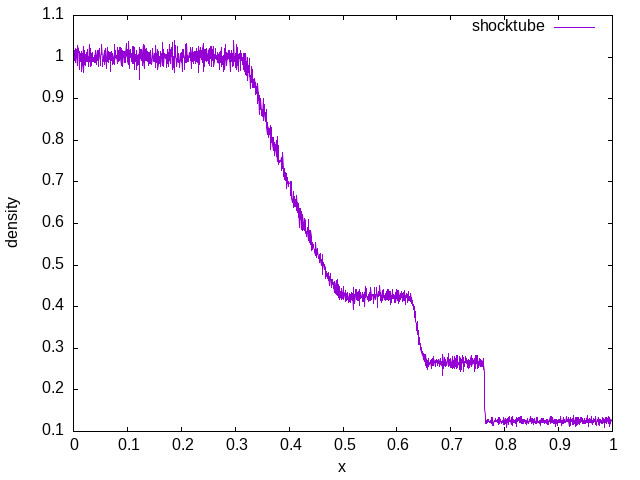
\includegraphics[width=0.78\linewidth]{shocktube.jpeg}
 \caption{\bphgpu で計算したSod衝撃波管の規格化セル密度。Monte Carlo粒子密度
 に、希薄波、接触不連続、衝撃波が現れている。}
 \label{fig:shocktube}
\end{figure}

図~\ref{fig:shocktube}の目的は限定的である。セルkey生成、共有並べ替え、segment
緩和、streaming、境界処理を合成し、数百万粒子規模の一連の計算を実行できることを
確認する。本テクニカルペーパーでは、この図から収束次数、誤差上界、他実装に対する
高速化を主張しない。同様に、backend間の性能測定も現在の範囲外とする。

\section{結論}

BPHのGPU実装における中心的な障害は、粒子局所の実行modelと、時間的に変化する
不均一なセル群上の緩和との不整合である。\bphgpu は、\massively v0.80を用いて
これを解決する。sort-by-keyはセルsegmentを連続化し、共有置換によってSoAの対応
を維持する。reduce-by-keyとscatterはdenseセルmomentを構成し、gatherはそれらを
粒子へ戻す。masked transformとcompactionは衝突・境界述語を実装する。この構成
では、セル単位の逐次loopも、粒子からセルへのatomic加算も必要ない。

緩和の導出は、このデータフローが保存すべき量を明らかにし、プリミティブlevelの
手順は補助的なライブラリ型に依存せずアルゴリズムを規定する。演算子テストによって
順序と集約の不変条件を確認し、450万粒子のSod計算によってGPU上に保持された一連の
cycleを実証した。本テクニカルペーパーの意図的に限定した実証範囲において、得られ
た結果は、CubeCLを通じて複数のGPU runtime familyへlowering可能な、再実装可能な
BPH並列分解である。

\begin{thebibliography}{99}

\bibitem{lucy1977}
L. B. Lucy, ``A Numerical Approach to the Testing of the Fission Hypothesis,''
\textit{The Astronomical Journal}, Vol. 82, pp. 1013--1024, 1977.
\url{https://doi.org/10.1086/112164}

\bibitem{gingold1977}
R. A. Gingold and J. J. Monaghan,
``Smoothed Particle Hydrodynamics: Theory and Application to Non-Spherical
Stars,'' \textit{Monthly Notices of the Royal Astronomical Society}, Vol. 181,
No. 3, pp. 375--389, 1977.
\url{https://doi.org/10.1093/mnras/181.3.375}

\bibitem{monaghan1992}
J. J. Monaghan, ``Smoothed Particle Hydrodynamics,''
\textit{Annual Review of Astronomy and Astrophysics}, Vol. 30, pp. 543--574,
1992.
\url{https://doi.org/10.1146/annurev.aa.30.090192.002551}

\bibitem{bird1994}
G. A. Bird, \textit{Molecular Gas Dynamics and the Direct Simulation of Gas
Flows}. Oxford University Press, 1994.

\bibitem{isaka2006}
H. Isaka, T. Matsuda, and H. M. J. Boffin,
``Application of Molecular Hydrodynamics to Astrophysical Flows:
Bondi--Hoyle--Lyttleton Accretion Flow,''
\textit{Progress of Theoretical Physics}, Vol. 116, No. 6, pp. 1069--1096,
2006.
\url{https://doi.org/10.1143/PTP.116.1069}

\bibitem{murata2008}
H. Murata, T. Matsuda, H. Isaka, Y. Ohsugi, and H. M. J. Boffin,
``Application of Molecular Hydrodynamics to Astrophysical Flows. II:
Unconditional Stability,'' \textit{Progress of Theoretical Physics}, Vol. 120,
No. 2, pp. 347--369, 2008.
\url{https://doi.org/10.1143/PTP.120.347}

\bibitem{isaka2010}
H. Isaka, T. Matsuda, and Y. Ohsugi,
``Improved Boltzmann Particle Method: Variable Number of Particles,''
\textit{Proceedings of the Japan Society of Fluid Mechanics Annual Meeting
2010}, p. 204, 2010 (in Japanese).
\url{https://cir.nii.ac.jp/crid/2051996266952625024}

\bibitem{bgk}
P. L. Bhatnagar, E. P. Gross, and M. Krook,
``A Model for Collision Processes in Gases. I. Small Amplitude Processes in
Charged and Neutral One-Component Systems,''
\textit{Physical Review}, Vol. 94, pp. 511--525, 1954.
\url{https://doi.org/10.1103/PhysRev.94.511}

\bibitem{crespo2011}
A. J. C. Crespo, J. M. Dominguez, A. Barreiro, M. G\'omez-Gesteira, and
B. D. Rogers, ``GPUs, a New Tool of Acceleration in CFD: Efficiency and
Reliability on Smoothed Particle Hydrodynamics Methods,''
\textit{PLOS ONE}, Vol. 6, No. 6, e20685, 2011.
\url{https://doi.org/10.1371/journal.pone.0020685}

\bibitem{su2012}
C.-C. Su, M. R. Smith, F.-A. Kuo, J.-S. Wu, C.-W. Hsieh, and K.-C. Tseng,
``Large-Scale Simulations on Multiple Graphics Processing Units (GPUs) for the
Direct Simulation Monte Carlo Method,''
\textit{Journal of Computational Physics}, Vol. 231, No. 23, pp. 7932--7958,
2012.
\url{https://doi.org/10.1016/j.jcp.2012.07.038}

\bibitem{massively}
A. Hayakawa, ``massively: Multi-platform GPU parallel algorithms for Rust,''
version 0.80, software library, 2026.
\url{https://github.com/akiradeveloper/massively}

\bibitem{cubecl}
Tracel AI, ``CubeCL: Multi-platform high-performance computing language
extension for Rust,'' source code.
\url{https://github.com/tracel-ai/cubecl}

\bibitem{sod1978}
G. A. Sod, ``A Survey of Several Finite Difference Methods for Systems of
Nonlinear Hyperbolic Conservation Laws,''
\textit{Journal of Computational Physics}, Vol. 27, No. 1, pp. 1--31, 1978.
\url{https://doi.org/10.1016/0021-9991(78)90023-2}

\end{thebibliography}

\end{document}
